% !TeX program = pdflatex
% Standalone source. Compile with pdfLaTeX; no external figures are required.
\documentclass[11pt,a4paper]{article}
\usepackage[margin=20mm]{geometry}
\usepackage[T1]{fontenc}
\usepackage{lmodern}
\usepackage{amsmath,amssymb,booktabs,array,xcolor,tikz,fancyhdr,hyperref,listings,pgfplots}
\usetikzlibrary{calc,arrows.meta}
\hypersetup{colorlinks=true,linkcolor=blue!50!black,urlcolor=blue!50!black}
\definecolor{accent}{HTML}{124E66}
\definecolor{pcol}{HTML}{A24021}
\definecolor{ncol}{HTML}{175A86}
\pagestyle{fancy}\fancyhf{}\fancyhead[L]{\small EE3032 / Fall 2021 / HW4}
\fancyhead[R]{\small CMOS logic}\fancyfoot[C]{\thepage}
\setlength{\headheight}{15pt}\setlength{\parindent}{0pt}\setlength{\parskip}{6pt}
\renewcommand{\arraystretch}{1.2}
\newcommand{\answer}[1]{\par\noindent\colorbox{accent!9}{\parbox{0.96\linewidth}{#1}}\par}
\newcommand{\AND}{\,}
\newcommand{\VDD}{V_{\mathrm{DD}}}
\newcommand{\VSS}{V_{\mathrm{SS}}}
% A conventional switch-level MOS symbol: continuous channel, insulated gate,
% and a gate bubble for pMOS. Bulk terminals are omitted, as explained below.
% Arguments: device id, x, y, gate literal, p or n. t/b are upper/lower terminals.
\newcommand{\MOS}[5]{
  \coordinate (#1) at (#2,#3);
  \coordinate (#1t) at ($(#1)+(0,.55)$);
  \coordinate (#1b) at ($(#1)+(0,-.55)$);
  \draw (#1t)--($(#1)+(0,.30)$)--($(#1)+(-.18,.30)$);
  \draw ($(#1)+(-.18,.34)$)--($(#1)+(-.18,-.34)$);
  \draw ($(#1)+(-.18,-.30)$)--($(#1)+(0,-.30)$)--(#1b);
  \draw ($(#1)+(-.35,.33)$)--($(#1)+(-.35,-.33)$);
  \def\type{#5}\def\ptype{p}
  \ifx\type\ptype
    \draw ($(#1)+(-.78,0)$)--($(#1)+(-.53,0)$);
    \draw ($(#1)+(-.465,0)$) circle (.065);
    \draw ($(#1)+(-.40,0)$)--($(#1)+(-.35,0)$);
  \else
    \draw ($(#1)+(-.78,0)$)--($(#1)+(-.35,0)$);
  \fi
  \node[anchor=east] at ($(#1)+(-.82,0)$) {$#4$};
  \node[anchor=west,font=\scriptsize] at ($(#1)+(.10,0)$) {#1};
}
% A transmission-gate instance; its two MOS devices are expanded on page 3.
\newcommand{\TG}[4]{
  \node[draw,rounded corners=1pt,minimum width=11mm,minimum height=6mm,
        fill=accent!5,font=\small] (#1) at (#2,#3) {$\mathrm{TG}_{#4}$};
}

\pgfplotsset{compat=1.18}
\lstset{basicstyle=\ttfamily\scriptsize,breaklines=true,frame=single,columns=fullflexible}
\begin{document}
\begin{center}{\LARGE\bfseries 2021 HW4}\\[4pt]{\large Two-input CMOS AND: Verified Pre-layout SPICE}\\[4pt]{\small EE3032 / Introduction to VLSI Design}\end{center}
\textbf{Provenance.} The original assignment and the supplied answers by Lin Yan-Yu were read first. The results below were independently derived, with the useful reference choices retained and improvements identified. Source details and hashes are in the year-level \texttt{SOURCES.md}.
\textbf{Requested HW4 scope.} This report completes part (a) and provides the pre-layout \texttt{.sp} circuit and testbench. Part (b)'s layout, extraction, DRC/LVS, and post-layout measurements are excluded as requested. No post-layout result is represented as a pre-layout measurement.

\section*{1. Circuit, sizes, and electrical conditions}
The assignment's labels are $F=\overline{AB}$ (the internal NAND output) and $Z=AB$ (the final AND output). The labeled $F$ gate terminals of MP5/MN6 connect to the NAND output. PMOS bulks are VDD and NMOS bulks are VSS.
\begin{center}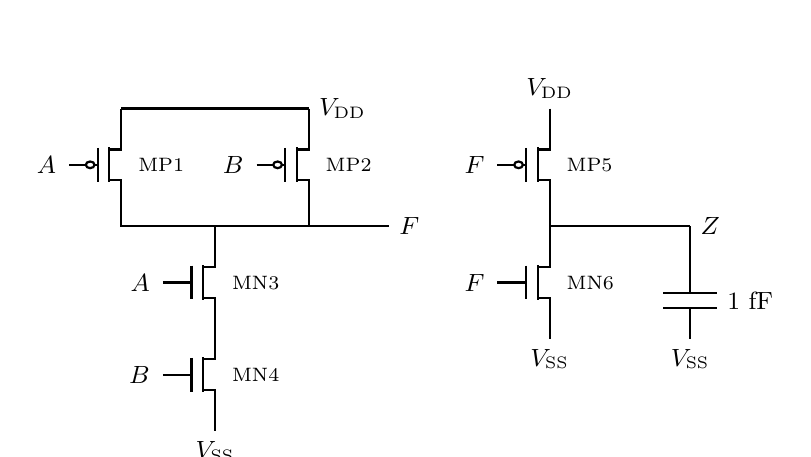
\begin{tikzpicture}[x=.85cm,y=.65cm,line width=.8pt,font=\small]
\MOS{MP1}{0}{6}{A}{p}\MOS{MP2}{2.8}{6}{B}{p}
\MOS{MN3}{1.4}{3.7}{A}{n}\MOS{MN4}{1.4}{1.9}{B}{n}
\draw (0,7.1)--(2.8,7.1) node[right] {$\VDD$};\draw (0,7.1)--(MP1t) (2.8,7.1)--(MP2t);
\draw (MP1b)--(0,4.8)--(4,4.8) node[right] {$F$};\draw (MP2b)--(2.8,4.8);
\draw (1.4,4.8)--(MN3t) (MN3b)--(MN4t);\draw (MN4b)--(1.4,.8) node[below] {$\VSS$};
\MOS{MP5}{6.4}{6}{F}{p}\MOS{MN6}{6.4}{3.7}{F}{n}
\draw (6.4,7.1) node[above] {$\VDD$}--(MP5t);
\draw (MP5b)--(MN6t);\draw (6.4,4.8)--(8.5,4.8) node[right] {$Z$};\draw (MN6b)--(6.4,2.6) node[below] {$\VSS$};
\draw (8.5,4.8)--(8.5,3.5);\draw (8.1,3.5)--(8.9,3.5) (8.1,3.2)--(8.9,3.2);\draw (8.5,3.2)--(8.5,2.6) node[below] {$\VSS$};\node[right] at (8.9,3.35) {1 fF};
\end{tikzpicture}\end{center}
\begin{center}\begin{tabular}{lrrl}\toprule
Devices&$W$ ($\mu$m)&$L$ ($\mu$m)&Role\\\midrule
MP1, MP2&3.00&0.18&Parallel NAND pull-up\\
MN3, MN4&2.00&0.18&Series NAND pull-down\\
MP5&3.00&0.18&Inverter pull-up\\
MN6&1.00&0.18&Inverter pull-down\\\bottomrule
\end{tabular}\qquad\begin{tabular}{cc|cc}\toprule
$A$&$B$&$F$&$Z$\\\midrule0&0&1&0\\0&1&1&0\\1&0&1&0\\1&1&0&1\\\bottomrule
\end{tabular}\end{center}
The NAND nMOS widths are doubled relative to MN6 to compensate approximately for its two-device stack. The pMOS width is three times MN6 to offset lower hole mobility. The prompt permits arbitrary sizes; this choice also enables a direct comparison with the supplied HW3 answer.
\textbf{Simulation conditions.} Actual PrimeSim HSPICE S-2021.09 win64, local CIC018 TT BSIM3 models, $\VDD=1.8$ V, $\VSS=0$, $25^\circ$C, and exactly 1 fF from $Z$ to ground. The input rise/fall time is 1 ns (0--100\%), the pulse width is 4 ns, and the period is 10 ns. The transient stop time is 32 ns and the requested output timestep is 2 ps.

\textbf{Voltage verification.} Sampling each initial state at 4 ns and the 11 state at 9 ns gives all four truth-table rows. All six samples pass with low $\le0.2$ V and high $\ge1.6$ V. The highest measured low value is below 12 $\mu$V; the lowest high value exceeds 1.79999 V.
\newpage
\section*{2. Propagation-delay measurements}
All delays are from the changing \emph{primary input} to the named output, at 50\% of VDD (0.9 V). For simultaneous changes in 00$\leftrightarrow$11, A and B have identical waveforms and either input gives the same trigger. For 01$\leftrightarrow$11, A changes; for 10$\leftrightarrow$11, B changes.
These three bidirectional cases enumerate every primary-input transition that changes $F$ or $Z$. The non-11-to-non-11 transitions do not create an intended output edge, so a propagation delay is not defined for them.
\begin{center}\begin{tabular}{lrrrr}\toprule
Case, first cycle&$F$: H--L&$F$: L--H&$Z$: H--L&$Z$: L--H\\
&ps&ps&ps&ps\\\midrule
00$\to$11$\to$00&132.577&41.723&71.163&161.193\\
01$\to$11$\to$01&55.385&133.104&164.004&85.929\\
10$\to$11$\to$10&47.248&162.474&193.646&77.026\\
\bottomrule\end{tabular}\end{center}
We also measure every edge in three consecutive cycles (36 measurements total). Taking the maximum separately for each output and direction gives:
\begin{center}\begin{tabular}{lcrcc}\toprule
Node&Direction&Worst delay (ps)&Initial AB&Cycle\\\midrule
F&HL&132.577&00&1\\
F&LH&162.579&10&2\\
Z&HL&193.782&10&2\\
Z&LH&161.193&00&1\\
\bottomrule\end{tabular}\end{center}
\textbf{Physical interpretation.} Both inputs rising together in the 00 case weakens the NAND discharge during the slow ramp, producing the largest $F$ falling delay. In the 10 case, B falls while A remains high: the internal stack node charges with F through the conducting upper device, increasing the effective capacitance. This gives the largest $F$ rising delay and, after the inverter, the largest $Z$ falling delay. The inverter adds delay, so $Z$ delays are input-to-Z values and are not just inverter-only delays.

\textbf{Reference comparison.} The supplied HW4 changes all six devices to $W/L=2/1\,\mu$m and includes a layout, so its pre-layout delays are larger (453/1050 ps at F and 1030/731 ps at Z). The prompt allows arbitrary sizes. We retain the faster verified HW3 sizing and the shared pre-layout circuit for this requested scope. The supplied layout and post-layout numbers are not part of this solution.
\newpage\section*{3. Deliverable pre-layout netlist and testbench}
\begin{lstlisting}
* 2021 CMOS AND gate; terminals A B F Z VDD VSS.
* F is the internal NAND output; Z is the final AND output.
* W/L in micrometres. PMOS bulk=VDD; NMOS bulk=VSS.
.subckt and2 a b f z vdd vss
mp1 f a vdd vdd p_18 w=3u l=.18u
mp2 f b vdd vdd p_18 w=3u l=.18u
mn3 f a x vss n_18 w=2u l=.18u
mn4 x b vss vss n_18 w=2u l=.18u
mp5 z f vdd vdd p_18 w=3u l=.18u
mn6 z f vss vss n_18 w=1u l=.18u
.ends and2
\end{lstlisting}

The standalone \texttt{testbench.sp} runs the simultaneous 00 case and directly includes \texttt{and2.sp}. The Python driver creates independent 00, 01, and 10 runs, preserving raw logs in the selected work directory. Each run measures all three cycles and validates the rail levels. The representative measurement definitions are:
\begin{lstlisting}
.measure tran f_hl1 trig v(a) val=.9 rise=1
+ targ v(f) val=.9 fall=1
.measure tran f_lh1 trig v(a) val=.9 fall=1
+ targ v(f) val=.9 rise=1
.measure tran z_lh1 trig v(a) val=.9 rise=1
+ targ v(z) val=.9 rise=1
.measure tran z_hl1 trig v(a) val=.9 fall=1
+ targ v(z) val=.9 fall=1
\end{lstlisting}
The circuit uses node 0 as the reference ground. Every supply terminal, bulk terminal, and the required output capacitance are explicit.
\textbf{Run command:}
\begin{lstlisting}
python reproduce.py --model D:/cic018.l --work PATH
# Optional: --hspice C:/synopsys/Hspice_S-2021.09/WIN64/hspice.com
\end{lstlisting}
Python uses only its standard library. Set \texttt{CIC018\_MODEL} and \texttt{HSPICE}, or use the command flags. The local process file is required and is not redistributed. A license failure stops the program; it cannot be mistaken for a successful simulation.
\textbf{Evidence files.} \texttt{results/delays.csv} contains all 36 actual delays; \texttt{logic\_levels.csv} contains six measured logic checks; \texttt{waveforms.csv} contains actual transient samples; \texttt{summary.json} records the conditions and maxima. The numerical tables above are generated from these data. Repeated-cycle variation is sub-picosecond and does not change the worst-case transition family.
\end{document}
